% Anonymised manuscript for double-anonymous review -- IIMB Management Review (BAICONF 2026, BAI2575)
% Overleaf: set Compiler = pdfLaTeX. Bibliography: biblatex-apa (APA 7) with Biber.
\documentclass[12pt,a4paper]{article}
% Shared preamble: IIMB Management Review submission (BAICONF 2026, BAI2575)
% Compile with pdfLaTeX + Biber (Overleaf: Menu > Compiler = pdfLaTeX; Biber runs automatically).
\usepackage[T1]{fontenc}
\usepackage[utf8]{inputenc}
\usepackage[british]{babel}
\usepackage{newtxtext,newtxmath}            % Times New Roman equivalent
\usepackage[a4paper,margin=1in]{geometry}
\usepackage{setspace}
\usepackage{amsmath,bm}
\usepackage{graphicx}
\usepackage{booktabs,tabularx,array,makecell,threeparttable}
\usepackage{pdflscape}
\usepackage[labelsep=period,font=small,labelfont=bf,justification=raggedright,singlelinecheck=false]{caption}
\captionsetup[figure]{name=Fig.}
\usepackage{xcolor}
\usepackage{microtype}
\usepackage{csquotes}
\usepackage[style=apa,backend=biber,uniquename=false]{biblatex}
\addbibresource{references.bib}
\usepackage[hidelinks]{hyperref}
\renewcommand{\cellalign}{tl}
\renewcommand{\theadalign}{tl}
\newcommand{\authorsto}[1]{\textbf{[AUTHORS TO COMPLETE: #1]}}
% Generated by R/run_all.R -- do not edit by hand
\newcommand{\nTrialsAll}{833}
\newcommand{\nAthAll}{215}
\newcommand{\nSessAll}{333}
\newcommand{\nTrials}{805}
\newcommand{\nAth}{212}
\newcommand{\nSess}{327}
\newcommand{\nTrialsS}{811}
\newcommand{\nLowcomMissing}{6}
\newcommand{\nFsLow}{60}
\newcommand{\ageMedian}{14.1}
\newcommand{\ageMin}{8.8}
\newcommand{\ageMax}{37.9}
\newcommand{\ageQone}{12.0}
\newcommand{\ageQthree}{16.8}
\newcommand{\nMinors}{164}
\newcommand{\pctMinors}{77}
\newcommand{\trialsPerAthMean}{3.8}
\newcommand{\trialsPerAthMax}{16}
\newcommand{\sessPerAthMedian}{1}
\newcommand{\sessPerAthMax}{6}
\newcommand{\trialsPerSessMedian}{2}
\newcommand{\jhMean}{28.2}
\newcommand{\jhSD}{8.4}
\newcommand{\lpfMean}{5.39}
\newcommand{\lpfSD}{1.97}
\newcommand{\lpfMin}{2.19}
\newcommand{\lpfMax}{14.88}
\newcommand{\lowcomTimeMedian}{0.24}
\newcommand{\varPCA}{37.3}
\newcommand{\varSPCA}{20.2}
\newcommand{\ldsPCA}{99.7}
\newcommand{\ldsSPCA}{96.4}
\newcommand{\peakPCA}{40}
\newcommand{\rLpfPCA}{0.39}
\newcommand{\rJhPCA}{0.13}
\newcommand{\rCtPCA}{$-$0.04}
\newcommand{\rCmdPCA}{0.01}
\newcommand{\rLdPCA}{$-$0.75}
\newcommand{\rtwoPCA}{7.7}
\newcommand{\rtwoSPCA}{19.1}
\newcommand{\cvPCA}{4.0}
\newcommand{\cvSPCA}{13.4}
\newcommand{\jhRatioPCA}{0.89}
\newcommand{\rpfRatioPCA}{1.01}
\newcommand{\jhLoPCA}{0.70}
\newcommand{\jhHiPCA}{1.06}
\newcommand{\betweenPCA}{29.6}
\newcommand{\withinPCA}{35.5}
\newcommand{\sessPCA}{34.9}
\newcommand{\betweenSPCA}{45.3}
\newcommand{\varPCB}{16.0}
\newcommand{\varSPCB}{16.6}
\newcommand{\ldsPCB}{99.9}
\newcommand{\ldsSPCB}{92.5}
\newcommand{\peakPCB}{26}
\newcommand{\rLpfPCB}{0.22}
\newcommand{\rJhPCB}{0.13}
\newcommand{\rCtPCB}{0.02}
\newcommand{\rCmdPCB}{0.00}
\newcommand{\rLdPCB}{$-$0.14}
\newcommand{\rtwoPCB}{2.7}
\newcommand{\rtwoSPCB}{5.3}
\newcommand{\cvPCB}{0.3}
\newcommand{\cvSPCB}{2.8}
\newcommand{\jhRatioPCB}{0.97}
\newcommand{\rpfRatioPCB}{1.05}
\newcommand{\jhLoPCB}{0.77}
\newcommand{\jhHiPCB}{1.16}
\newcommand{\betweenPCB}{21.4}
\newcommand{\withinPCB}{61.6}
\newcommand{\sessPCB}{17.0}
\newcommand{\betweenSPCB}{18.7}
\newcommand{\varPCC}{12.6}
\newcommand{\varSPCC}{15.1}
\newcommand{\ldsPCC}{99.5}
\newcommand{\ldsSPCC}{3.7}
\newcommand{\peakPCC}{16}
\newcommand{\rLpfPCC}{0.39}
\newcommand{\rJhPCC}{0.34}
\newcommand{\rCtPCC}{0.00}
\newcommand{\rCmdPCC}{$-$0.14}
\newcommand{\rLdPCC}{$-$0.32}
\newcommand{\rtwoPCC}{13.1}
\newcommand{\rtwoSPCC}{68.3}
\newcommand{\cvPCC}{11.8}
\newcommand{\cvSPCC}{66.4}
\newcommand{\jhRatioPCC}{0.95}
\newcommand{\rpfRatioPCC}{1.00}
\newcommand{\jhLoPCC}{0.74}
\newcommand{\jhHiPCC}{1.13}
\newcommand{\betweenPCC}{22.9}
\newcommand{\withinPCC}{74.8}
\newcommand{\sessPCC}{2.3}
\newcommand{\betweenSPCC}{26.5}
\newcommand{\varPCD}{8.9}
\newcommand{\varSPCD}{10.2}
\newcommand{\ldsPCD}{99.3}
\newcommand{\ldsSPCD}{80.2}
\newcommand{\peakPCD}{9}
\newcommand{\rLpfPCD}{0.45}
\newcommand{\rJhPCD}{0.24}
\newcommand{\rCtPCD}{0.15}
\newcommand{\rCmdPCD}{$-$0.18}
\newcommand{\rLdPCD}{$-$0.04}
\newcommand{\rtwoPCD}{9.1}
\newcommand{\rtwoSPCD}{17.8}
\newcommand{\cvPCD}{6.3}
\newcommand{\cvSPCD}{15.1}
\newcommand{\jhRatioPCD}{1.17}
\newcommand{\rpfRatioPCD}{1.05}
\newcommand{\jhLoPCD}{0.81}
\newcommand{\jhHiPCD}{1.44}
\newcommand{\betweenPCD}{10.0}
\newcommand{\withinPCD}{69.6}
\newcommand{\sessPCD}{20.3}
\newcommand{\betweenSPCD}{31.6}
\newcommand{\cumFour}{74.8}
\newcommand{\cumFourS}{62.2}
\newcommand{\cumTen}{93.8}
\newcommand{\rtwoRange}{2.7--13.1}
\newcommand{\unexplRange}{86.9--97.3}
\newcommand{\cvRange}{0.3--11.8}
\newcommand{\oneTrialRange}{4.3--17.8}
\newcommand{\athMeanRange}{5.4--21.2}
\newcommand{\adjRange}{2.0--12.4}
\newcommand{\rtwoLandingSRange}{5.3--19.1}
\newcommand{\unexplSRange}{31.7--94.7}
\newcommand{\lpfCorRange}{0.22--0.45}
\newcommand{\ctAbsMax}{0.15}
\newcommand{\cmdAbsMax}{0.18}
\newcommand{\vendorAbsMax}{0.34}
\newcommand{\rLpfSPCA}{0.71}
\newcommand{\rLdSPCA}{$-$0.57}
\newcommand{\ldsSPCCtakeoff}{96.3}
\newcommand{\rCtSPCC}{$-$0.79}
\newcommand{\rRpfSPCC}{0.77}
\newcommand{\jhBandN}{82}
\newcommand{\jhBandAth}{51}
\newcommand{\jhBandLo}{26.0}
\newcommand{\jhBandHi}{28.2}
\newcommand{\jhBandMean}{27.1}
\newcommand{\jhBandSD}{0.65}
\newcommand{\rpfBandN}{81}
\newcommand{\rpfBandAth}{58}
\newcommand{\rpfBandLo}{2.25}
\newcommand{\rpfBandHi}{2.32}
\newcommand{\jhBandSDfactor}{13}
\newcommand{\wholeJh}{1.01}
\newcommand{\wholeRpf}{1.00}
\newcommand{\wholeJhS}{1.01}
\newcommand{\rpfRatioRange}{1.00--1.05}
\newcommand{\jhRatioRange}{0.89--1.17}
\newcommand{\jhRatioOtherRange}{0.95--1.17}
\newcommand{\jhRatioSPCA}{0.82}
\newcommand{\jhLoSPCA}{0.69}
\newcommand{\jhHiSPCA}{0.96}
\newcommand{\bwPCARange}{0.87--0.89}
\newcommand{\bwAllRange}{0.84--1.17}
\newcommand{\betweenRange}{10.0--29.6}
\newcommand{\withinRange}{35.5--74.8}
\newcommand{\sessRange}{2.3--34.9}
\newcommand{\nFsLowAnalysed}{59}
\newcommand{\varShareTakeoff}{7.1}
\newcommand{\varShareLanding}{92.9}
\newcommand{\varShareTakeoffS}{31.0}
\newcommand{\rpfRatioSPCC}{0.74}
\newcommand{\rpfLoSPCC}{0.57}
\newcommand{\rpfHiSPCC}{0.87}
\newcommand{\nAthMultiSess}{83}
\newcommand{\baCIUpperRange}{23--47}
\newcommand{\baLoPCA}{13}
\newcommand{\baHiPCA}{47}
\newcommand{\baCIMaxUpper}{47}
\newcommand{\baAgeAdjRange}{7.1--28.2}
\newcommand{\baAgeMaxChange}{7.1}
\newcommand{\baAgePCA}{28.2}
\newcommand{\landRtwoPCA}{56.8}
\newcommand{\landRtwoOtherRange}{5.1--24.0}
\newcommand{\sbTrials}{3}
\newcommand{\sbPCA}{0.85}
\newcommand{\sbRange}{0.50--0.85}
\newcommand{\sdMinorPCA}{6.5}
\newcommand{\sdAdultPCA}{8.9}
\newcommand{\nTrialsMinor}{598}
\newcommand{\nZeroCmd}{1}
\newcommand{\nLowBrake}{17}
\newcommand{\nBoot}{2,000}
\newcommand{\seedValue}{2026}
\newcommand{\nRepro}{42}
\newcommand{\nReproTotal}{42}

% Figure captions (greyscale figures; numbers come from numbers.tex)
\newcommand{\capMean}{(A) Mean body-weight-normalised vertical force (line) $\pm$ 1 SD (shaded) of the \nTrials{} analysed countermovement jumps. The take-off phase (movement onset to take-off) and the landing phase (touch-down to the lowest point of the centre of mass, COM) were each time-normalised to 0--100\% and concatenated; flight is omitted. The dotted line marks body weight. (B) Variance explained by each of the first ten principal components (bars) and cumulatively (line); the dashed line marks the four retained components.}
\newcommand{\capPCs}{Interpretation of the four retained principal components (main analysis). Each panel shows the mean curve (thin grey line) and the mean curve plus (solid black line) or minus (dashed black line) two standard deviations of the component score. Values below zero in the reconstructions are an artefact of adding a linear component to the mean and do not correspond to observed trials. The vertical line separates the take-off and landing phases.}
\newcommand{\capBand}{Trials matched on jump height do not share a common force--time curve. (A) Curves of the \jhBandN{} trials between the 45th and 55th percentiles of jump height (\jhBandMean{} $\pm$ \jhBandSD{}\,cm), shaded from light grey (low) to black (high) by their PC1 score. (B) Ratio of the standard deviation of each component score among trials matched on jump height (black circles) or on relative concentric peak force (grey triangles) to that in the full sample, with athlete-level bootstrap 95\% confidence intervals. A ratio of 1 indicates that matching on the metric leaves curve-shape variation unchanged.}
\newcommand{\capRtwo}{Proportion of the variance of each component score explained by the four vendor metrics, age and body mass, under four evaluation schemes (bars from black to white: in-sample, athlete-grouped cross-validation, one trial per athlete, athlete means), for the main landing definition (left) and the 1-s landing window (right). CV, cross-validation with athletes allocated to folds.}
\newcommand{\capWindow}{Sensitivity analysis with the landing phase ending 1\,s after touch-down: mean curve (thin grey line) and the mean curve plus (solid black line) or minus (dashed black line) two standard deviations of each retained component. Under this definition PC3 is located almost entirely in the take-off phase (\ldsSPCCtakeoff\% of its squared loading) and describes the duration and amplitude of the propulsive force.}

\graphicspath{{figures/}}
\setlength{\emergencystretch}{2em}
% Testing period: min--max recorded date (IST) of the 327 analysed sessions in the raw export (derived 13 Nov 2026)
\newcommand{\testPeriod}{November 2022 and April 2026}
% Title, short title, abstract, keywords and extended summary (anonymised; IIMB MR page 2 requirements)
\newcommand{\papertitle}{Revealing hidden jump strategies beyond conventional force-plate metrics}
\newcommand{\shorttitle}{Hidden strategies in jump curves}


\usepackage{lineno}
\begin{document}
\doublespacing
\begin{center}
{\Large\bfseries \papertitle\par}
\medskip
{\normalsize Short title: \shorttitle\par}
\end{center}
\bigskip
\noindent\textbf{Abstract}\par\smallskip
\noindent Force-plate software summarises each countermovement jump (CMJ) with a few vendor metrics, and athletes with similar values are treated as equivalent. We tested that assumption with \nTrials{} routine CMJ trials from \nAth{} male footballers in India. Principal component analysis of body-weight-normalised take-off and landing force--time curves retained four components (\cumFour\% of variance), concentrated in the landing phase. Trials matched on jump height or relative peak force varied nearly as much as the full sample; vendor metrics, age and body mass explained \rtwoRange\% of each component. Most of this variation arose within athletes, so landing information needs averaging over trials and sessions.

\medskip
\noindent\textbf{Keywords:} Countermovement jump; Principal component analysis; Force--time curve; Force plates; Athlete monitoring; Landing; Sports analytics; Football

\clearpage
\noindent\textbf{Extended summary}\par\smallskip
High-performance centres invest in force plates and test athletes routinely, yet decisions about those athletes usually rest on a small number of vendor-computed values, such as jump height and peak force. Athletes with similar values are then treated as though they had jumped in the same way. This study asks whether that inference holds and how much of the recorded information those values leave unused.

The analysis used \nTrials{} countermovement jumps from \nAth{} male football players tested during routine monitoring at a private sports physiotherapy and performance centre in India. Each force--time curve was normalised to body weight; the take-off and landing phases were time-normalised separately and concatenated, and principal component analysis identified the main modes of variation. The dispersion of curve shapes among jumps matched on jump height, or on relative peak force, was compared with that of the whole sample, and the share of each mode explained by four vendor metrics, age and body mass was estimated.

Four components explained \cumFour\% of curve variance, and all four lay almost entirely in the landing phase; the first described how quickly the athlete arrested the fall. Jumps matched on jump height were scarcely more alike in shape than jumps in general, and matching on relative peak force had no discernible effect. The conventional metrics, age and body mass explained \rtwoRange\% of each component (\cvRange\% out of sample). Between-athlete differences accounted for \betweenRange\% of component variance, indicating that much of the variation was trial-specific. With a fixed 1-s landing window, a take-off component emerged that the metrics largely explained.

For those who manage sports-science programmes, the landing is recorded in every jump at no additional cost. Simple landing descriptors could be added to routine reports, provided that decisions rest on several trials rather than on a single landing.

\clearpage
\linenumbers
\section{Introduction}
\label{sec:intro}

The countermovement jump (CMJ) performed on force platforms is one of the most widely used tests in team sports. It is quick to administer, places little demand on the athlete and is sensitive to training and to neuromuscular fatigue \parencite{claudino2017,gathercole2015}. Commercial systems detect the phases of the jump automatically and return a large number of variables for every trial, including jump height, peak forces, phase impulses and phase durations \parencite{mcmahon2018}. In routine practice, however, decisions rest on a small subset of these values. Practitioners are advised to select a limited set of metrics suited to the question at hand, whether performance profiling, fatigue monitoring or return to sport \parencite{bishop2023}. Athletes with similar values on those metrics are then treated, implicitly, as having jumped in a similar way.

This practice raises a measurement question that is common to many data-rich organisations: whether the summary indicators produced by a measurement system retain the information that matters for decisions, or whether part of the recorded signal is discarded. In sport, the question is sharpened by what is known about human movement. The same outcome can be achieved through different coordinative solutions, and variability in task execution is regarded as a functional property of the neuromusculoskeletal system rather than as noise \parencite{davids2003,bartlett2007,preatoni2013}. It is therefore plausible that two jumps of equal height are produced, and absorbed, in quite different ways.

The present study examines this possibility in routinely collected force-plate data from male footballers in India. It analyses the complete take-off and landing force--time curve of each jump, rather than a set of pre-selected points, and asks three questions. First, what are the principal modes of variation of the curve, and how can they be interpreted biomechanically? Second, are trials that are matched on jump height, or on relative concentric peak force, more alike in curve shape than the sample as a whole? Third, how much of each mode of variation is explained by four conventional vendor metrics together with age and body mass, when the repeated trials of each athlete are taken into account? The study also partitions curve-shape variation between athletes, sessions and trials, and examines the sensitivity of the conclusions to the definition of the landing phase.

The study contributes to the literature in three ways. It quantifies directly, through a matched-band design, how far conventional metrics fail to capture curve shape; it incorporates the landing phase, which is recorded in every trial but is usually discarded; and it evaluates explained variance with schemes that respect the repeated-measures structure of monitoring data. The remainder of the paper is organised as follows. Section~\ref{sec:lit} reviews the relevant literature, Section~\ref{sec:methods} describes the data and methods, and Section~\ref{sec:results} presents the results. Section~\ref{sec:discussion} discusses the findings, Section~\ref{sec:implications} sets out managerial and practical implications, Section~\ref{sec:limitations} notes limitations and directions for further research, and Section~\ref{sec:conclusion} concludes.

\section{Literature review}
\label{sec:lit}

\subsection{Discrete force-plate metrics in athlete monitoring}

For the vertical jump, no single kinetic or temporal variable fully accounts for performance \parencite{dowling1993}. Athletes of different jumping ability differ in how force is distributed across the unweighting, braking and propulsion phases \parencite{sole2018}; force--time characteristics differ by sex and sport \parencite{laffaye2014}; and the manner in which force is produced within individual sub-phases is related to performance \parencite{harry2018}. Recent work distinguishes performance metrics, such as jump height, from strategy variables, such as countermovement depth and phase durations \parencite{harry2024}. Strategy-based CMJ variables have been shown to detect fatigue when jump height does not \parencite{gathercole2015}, and analyses of whole force--, velocity-- and power--time curves have described training-induced changes across the curve rather than at single points \parencite{cormie2009}. These findings suggest that the metrics reported routinely provide an incomplete description of how a jump is performed.

\subsection{Waveform analysis of force--time curves}

Waveform methods describe the whole curve without requiring variables to be selected in advance. Principal component analysis (PCA) of time-normalised waveforms, and its functional counterpart, decompose a set of curves into a small number of orthogonal modes of variation, each with a score for every trial \parencite{jolliffe2002,ramsay2005,jolliffe2016}. In biomechanics, these methods have been applied to gait waveforms in knee osteoarthritis \parencite{deluzio2007}, knee kinematics in the vertical jump \parencite{ryan2006}, running kinematics in Achilles tendinopathy \parencite{donoghue2008} and on-water rowing \parencite{warmenhoven2019}, and principled approaches to interpreting the components have been proposed \parencite{brandon2013}. For vertical jumps, dimensionality-reduction techniques describe performance-related aspects of the curve better than discrete points \parencite{richter2014b}, principal component waveform analysis identifies improvements in jump performance \parencite{floria2019}, and alignment of curves on biomechanical events increases the information that can be extracted from them \parencite{richter2014a,moudy2018}.

\subsection{The landing phase and the research gap}

The landing that follows every CMJ is usually discarded, although it is recorded on the same plates within the same trial. Landing kinetics are nonetheless of independent interest. Stiff landings with high vertical forces have been associated with anterior cruciate ligament injury risk in young female athletes \parencite{leppanen2017}, jumping and landing variables have some utility as predictors of injury \parencite{pedley2020}, and CMJ landing characteristics change with the effort that athletes perceive themselves to be making \parencite{hite2025}. Moreover, although waveform studies show that curves carry information beyond discrete variables, the extent to which routinely reported metrics fail to capture curve shape has rarely been quantified directly, and, to the authors' knowledge, it has not been examined by asking whether jumps matched on those metrics have matched curves. Routinely collected data from youth football, in which large numbers of tests are performed under field conditions, provide an opportunity to address this question at a realistic scale.

\section{Data and methodology}
\label{sec:methods}

\subsection{Research design}

The study is a retrospective, cross-sectional analysis of routinely collected force-plate data. The analysis proceeded in five stages. Raw force-plate exports were first de-identified and screened with pre-specified quality-control rules. Each retained trial was then normalised to body weight, and its take-off and landing phases were time-normalised and concatenated into a single curve. PCA of these curves yielded component scores for every trial. The scores were subsequently used in three analyses: dispersion among trials matched on conventional metrics, the variance explained by those metrics, and the partition of variance between athletes, sessions and trials. Finally, the complete analysis was repeated with an alternative definition of the landing phase. Quality-control rules, phase definitions, the number of retained components and the matched-band definition were fixed before any result was examined, and no choice was tuned on the data.

\subsection{Data source and participants}

The data comprise countermovement jumps performed by male football players during routine testing at a private sports physiotherapy and performance centre in India between \testPeriod. The data were made available to the authors under a signed non-disclosure and data-sharing agreement between the centre and the authors. All CMJ trials of male football players available through the vendor's external application programming interface were extracted (\nTrialsAll{} trials from \nAthAll{} athletes in \nSessAll{} sessions). Before analysis, athletes, tests and trials were replaced by pseudonymous codes. The analysis files contain no names, team names, dates of birth, test dates or vendor identifiers, and the key linking codes to athletes is held separately by the first author. Age at test was computed before de-identification and rounded to 0.1 year. Of the \nAth{} analysed athletes, \nMinors{} (\pctMinors\%) were under 18 years of age at their first analysed test. \authorsto{name of the ethics committee, approval number and date; consent of athletes and parental or guardian consent for those under 18 years, or the waiver of consent for secondary use of routine monitoring data; and a statement that the study conformed to the Declaration of Helsinki}

\subsection{Instrumentation and test protocol}

Trials were recorded on VALD ForceDecks dual force platforms (VALD Performance, Brisbane, Australia), which record the vertical ground reaction force under each foot; total vertical force was the sum of the two plates. Most trials were sampled at 1000\,Hz; \nFsLow{} trials were recorded at 500\,Hz, which does not affect the analysis because every phase was resampled to a common grid (Section~\ref{sec:curves}). Each session contained one or more trials (median \trialsPerSessMedian{} per session), and athletes contributed a median of \sessPerAthMedian{} session (maximum \sessPerAthMax). Tests were administered by the centre's staff as part of routine assessments rather than under a research protocol; the warm-up, verbal instructions and rest intervals were therefore not recorded with the data, and landing technique was not standardised. The vendor software identified movement onset and returned, for every trial, the four metrics used in this study, namely jump height (from flight time), concentric peak force, eccentric braking impulse and concentric impulse over the first 100\,ms of the concentric phase, together with contraction time, flight time, countermovement depth and peak landing force, which were used only for interpretation.

\subsection{Event detection and phase definitions}
\label{sec:events}

Three events were taken from the vendor output: movement onset $t_{\mathrm{on}}$; take-off $t_{\mathrm{to}} = t_{\mathrm{on}} + T_{\mathrm{c}}$, where $T_{\mathrm{c}}$ is the contraction time; and touch-down $t_{\mathrm{td}} = t_{\mathrm{to}} + T_{\mathrm{f}}$, where $T_{\mathrm{f}}$ is the flight time \parencite{owen2014,mcmahon2018,harry2020}. The take-off phase ran from $t_{\mathrm{on}}$ to $t_{\mathrm{to}}$. In the main analysis, the landing phase ran from touch-down to the lowest point of the centre of mass (COM), that is, the instant at which the downward velocity acquired during the fall is first brought to zero, which marks the end of impact absorption. The vertical velocity of the COM was obtained by integrating the impulse--momentum relationship from touch-down \parencite{linthorne2001,street2001}:
\begin{equation}
v(t) = -\frac{g\,T_{\mathrm{f}}}{2} + \int_{t_{\mathrm{td}}}^{t} \frac{F(s) - m g}{m}\,\mathrm{d}s,
\qquad
t_{\mathrm{lc}} = \min\{\, t > t_{\mathrm{td}} : v(t) \ge 0 \,\},
\label{eq:velocity}
\end{equation}
where $F$ is the total vertical force, $m$ the body mass, $g = 9.81$\,m\,s$^{-2}$, and the initial value is the touch-down velocity implied by a symmetrical flight. The landing phase in the main analysis was therefore $[t_{\mathrm{td}}, t_{\mathrm{lc}}]$. Because no consensus definition of the end of the CMJ landing exists, a sensitivity analysis used a fixed window from touch-down to 1\,s after touch-down, which is the end of the vendor's trial record.

\subsection{Quality control}

Five rules were applied in order (Table~\ref{tab:qc}). Trials were excluded if the vendor body mass was missing or invalid (R1), because every curve is divided by body weight; if the mass estimated from quiet stance before the jump differed from the vendor body mass by more than 5\% (R2), which indicates an incorrectly entered mass or an athlete who was not still; if the mean force recorded during flight exceeded 50\,N (R3), which indicates contact with the plate during flight or an event-detection error; if any of the four metrics or age was missing (R4); or, in the main analysis only, if the lowest point of the COM could not be identified within the recorded landing (R5).

% Generated from package/output/paper_tables_latex/tab1_qc.tex (R pipeline); only layout changed.
\begin{table}[tbp]
\centering
\begin{threeparttable}
\caption{Quality-control flow (main analysis).}
\label{tab:qc}
\small
\begin{tabular*}{\linewidth}{@{\extracolsep{\fill}}lrrr@{}}
\toprule
Step & Trials & Sessions & Athletes \\
\midrule
All male football CMJ trials & 833 & 333 & 215 \\
R1: valid body mass & 828 & 329 & 212 \\
R2: quiet-stance mass within 5\% of body mass & 813 & 328 & 212 \\
R3: no force on plate during flight & 811 & 327 & 212 \\
R4: complete metrics and age & 811 & 327 & 212 \\
R5: end of landing (lowest COM) found & 805 & 327 & 212 \\
\bottomrule
\end{tabular*}
\begin{tablenotes}[flushleft]\footnotesize
\item \textit{Note.} Rules R1--R4 were fixed before any result was examined; R5 applies only to the main landing definition (touch-down to the lowest point of the centre of mass), and the 1-s landing window therefore retained \nTrialsS{} trials. Sessions are test occasions on which an athlete performed one or more trials. COM = centre of mass.
\end{tablenotes}
\end{threeparttable}
\end{table}


\subsection{Curve construction}
\label{sec:curves}

Force was expressed in multiples of body weight, $\tilde F(t) = F(t)/(m g)$, so that curves of athletes of different mass are directly comparable and a value of one corresponds to quiet standing. Each phase $[t_a, t_b]$ was then resampled by linear interpolation at 101 equally spaced instants:
\begin{equation}
\tilde F^{(p)}_k = \tilde F\!\left(t_a + \tfrac{k}{100}\,(t_b - t_a)\right), \qquad k = 0, 1, \ldots, 100.
\end{equation}
This procedure aligns take-off at the end of the first block and touch-down at the start of the second, a simple form of landmark registration \parencite{ramsay2005,richter2014a,moudy2018}. Time-normalising the whole trial to a single scale was rejected because the same event would then fall at different percentages in different trials, so that differences in timing would be confounded with differences in shape. The flight phase was omitted. During flight the force is zero, so this portion of the curve carries no information about force production other than its duration, which determines flight-time jump height \parencite{linthorne2001}; retaining it would allow the analysis to recover a conventional metric from the length of a block. Each trial was therefore represented by the vector $\mathbf{x}_i \in \mathbb{R}^{202}$ formed by the take-off block followed by the landing block.

\subsection{Principal component analysis}

PCA was applied to the $n \times 202$ matrix of curves \parencite{jolliffe2002,jolliffe2016}. Because all points share the same unit, the analysis used the covariance matrix of the centred curves without scaling:
\begin{equation}
\mathbf{S} = \frac{1}{n-1}\sum_{i=1}^{n}(\mathbf{x}_i - \bar{\mathbf{x}})(\mathbf{x}_i - \bar{\mathbf{x}})^{\top} = \mathbf{V}\boldsymbol{\Lambda}\mathbf{V}^{\top},
\qquad
z_{ik} = \mathbf{v}_k^{\top}(\mathbf{x}_i - \bar{\mathbf{x}}),
\end{equation}
where $\mathbf{v}_k$ is the $k$th loading vector (of unit length), $\lambda_k$ its eigenvalue and $z_{ik}$ the score of trial $i$ on component $k$; the proportion of variance explained by component $k$ is $\lambda_k / \sum_j \lambda_j$. Four components were retained, as specified before the analysis, and the sign of each loading vector was fixed so that its largest absolute element was positive. Components were interpreted in three ways: by reconstructing the curves $\bar{\mathbf{x}} \pm 2\sqrt{\lambda_k}\,\mathbf{v}_k$, which show the effect of a two-standard-deviation change in the score \parencite{brandon2013,warmenhoven2019}; by the share of each component located in the landing phase, $\sum_{j \in \mathcal{L}} v_{jk}^2$, where $\mathcal{L}$ indexes the 101 landing points; and by Pearson correlations of the scores with interpretable descriptors (peak landing force relative to body weight, landing duration $t_{\mathrm{lc}} - t_{\mathrm{td}}$, contraction time, countermovement depth, the four vendor metrics, age and body mass).

\subsection{Matched-band dispersion}

To test whether equal conventional scores imply equal curves (the second research question), trials between the 45th and 55th percentiles of jump height were selected, together with, separately, trials between the same percentiles of concentric peak force relative to body weight. For each component, the dispersion ratio
\begin{equation}
\rho_k = \frac{\mathrm{SD}(z_{k} \mid i \in \mathcal{B})}{\mathrm{SD}(z_{k})}
\end{equation}
compares the standard deviation of the score among trials in band $\mathcal{B}$ with that in the full sample. A ratio close to one indicates that fixing the metric does not make curves more alike, whereas a ratio well below one indicates that the metric constrains curve shape. The same comparison was made for the whole curve as $\rho = \{\mathrm{tr}(\mathbf{S}_{\mathcal{B}})/\mathrm{tr}(\mathbf{S})\}^{1/2}$, where $\mathbf{S}_{\mathcal{B}}$ is the covariance matrix within the band. Because athletes contributed several trials, 95\% confidence intervals for $\rho_k$ were obtained from \nBoot{} bootstrap resamples of athletes, each resample including all trials of the selected athletes, with band limits held fixed \parencite{efron1993}.

\subsection{Variance explained by conventional metrics}

For the third research question, each component score was regressed by ordinary least squares on the four vendor metrics, age and body mass:
\begin{equation}
z_{ik} = \beta_{0k} + \sum_{q=1}^{6}\beta_{qk}\,w_{iq} + \varepsilon_{ik},
\end{equation}
and the coefficient of determination $R^2_k$ was taken as the share of the component explained, so that $1 - R^2_k$ is the share left unexplained. Because in-sample $R^2$ is optimistic and trials of the same athlete are not independent, three further evaluations were made. In athlete-grouped five-fold cross-validation, athletes rather than trials were allocated to folds \parencite{roberts2017}, and the out-of-sample coefficient was computed as $1 - \sum_i (z_{ik} - \hat z^{(-f)}_{ik})^2 / \sum_i (z_{ik} - \bar z_k)^2$, where $\hat z^{(-f)}_{ik}$ is the prediction from the model fitted without the fold containing trial $i$. The regressions were also refitted with one randomly selected trial per athlete and with athlete means of all variables.

\subsection{Structure of repeated measurements}

To establish whether component scores describe stable characteristics of athletes or vary from trial to trial, each score was decomposed with a three-level random-intercept model,
\begin{equation}
z_{ajt} = \mu + a_a + b_{aj} + e_{ajt}, \quad a_a \sim N(0, \sigma^2_{\mathrm{A}}),\; b_{aj} \sim N(0, \sigma^2_{\mathrm{S}}),\; e_{ajt} \sim N(0, \sigma^2_{\mathrm{T}}),
\end{equation}
for trial $t$ of session $j$ of athlete $a$, fitted by restricted maximum likelihood \parencite{pinheiro2000}. The shares of $\sigma^2_{\mathrm{A}}$, $\sigma^2_{\mathrm{S}}$ and $\sigma^2_{\mathrm{T}}$ in the total variance are reported; the between-athlete share is an intraclass correlation coefficient for a single trial \parencite{hopkins2000,koo2016}.

\subsection{Sensitivity analyses and software}

The complete analysis was repeated with the 1-s landing window, and the width of the jump-height band was varied (40th--60th percentile, and median $\pm$ 1\,cm and $\pm$ 2\,cm). All analyses were run by a single R script in R 4.5.3 \parencite{rcore2026} with the packages dplyr, tidyr, ggplot2 \parencite{wickham2016}, patchwork and nlme \parencite{pinheiro2000}; every random step (cross-validation folds, one-trial selection and the bootstrap) used seed \seedValue. The script writes every table, figure and number reported in this article. A preliminary version of the analysis was summarised in a conference abstract; rerunning the script from the de-identified data reproduced all \nReproTotal{} values checked against the corresponding analysis report. Statistical reporting followed recommendations for sports medicine and exercise science \parencite{hopkins2009}.

\section{Results}
\label{sec:results}

\subsection{Sample characteristics}

Of \nTrialsAll{} trials, \nTrials{} trials from \nAth{} athletes in \nSess{} sessions met all quality-control criteria (Table~\ref{tab:qc}); the 1-s landing window retained \nTrialsS{} trials, because the lowest point of the COM could not be identified in \nLowcomMissing{} trials. The median age of athletes at their first analysed test was \ageMedian{} years (interquartile range \ageQone--\ageQthree{}; range \ageMin--\ageMax), and athletes contributed \trialsPerAthMean{} trials on average (maximum \trialsPerAthMax). Mean jump height was \jhMean{} $\pm$ \jhSD{}\,cm, and peak landing force ranged from \lpfMin{} to \lpfMax{} times body weight (Table~\ref{tab:desc}).

% Generated from package/output/paper_tables_latex/tab2_descriptives.tex (R pipeline); only layout changed.
\begin{table}[tbp]
\centering
\begin{threeparttable}
\caption{Characteristics of the analysed sample (\nTrials{} trials, \nAth{} athletes).}
\label{tab:desc}
\footnotesize
\setlength{\tabcolsep}{3pt}
\begin{tabular*}{\linewidth}{@{\extracolsep{\fill}}>{\raggedright\arraybackslash}p{0.30\linewidth}rlll@{}}
\toprule
Variable & $n$ & Mean $\pm$ SD & Median (IQR) & Range \\
\midrule
Age at first test (years) & 212 & 16.01 $\pm$ 5.94 & 14.10 (12.00--16.80) & 8.80--37.90 \\
Body mass at first test (kg) & 212 & 53.31 $\pm$ 15.90 & 51.73 (40.86--64.03) & 25.03--95.97 \\
Jump height, flight time (cm) & 805 & 28.19 $\pm$ 8.43 & 26.96 (21.62--34.69) & 8.54--51.47 \\
Concentric peak force (N) & 805 & 1269.26 $\pm$ 420.74 & 1227.01 (923.47--1582.99) & 473.52--3073.22 \\
Concentric peak force ($\times$\,BW) & 805 & 2.35 $\pm$ 0.38 & 2.29 (2.11--2.51) & 1.65--4.70 \\
Eccentric braking impulse (N\,s) & 805 & 27.80 $\pm$ 15.43 & 24.60 (16.59--35.70) & 0.00--95.18 \\
Concentric impulse, first 100 ms (N\,s) & 805 & 62.24 $\pm$ 26.66 & 58.70 (41.76--79.14) & 1.51--187.93 \\
Peak landing force ($\times$\,BW) & 805 & 5.39 $\pm$ 1.97 & 4.97 (3.88--6.67) & 2.19--14.88 \\
Contraction time (s) & 805 & 0.78 $\pm$ 0.19 & 0.77 (0.66--0.90) & 0.31--1.48 \\
Countermovement depth (cm) & 805 & $-$26.55 $\pm$ 9.90 & $-$27.13 ($-$33.55--$-$20.71) & $-$52.39--0.00 \\
Touch-down--lowest COM (s) & 805 & 0.25 $\pm$ 0.11 & 0.24 (0.15--0.31) & 0.07--0.93 \\
Trials per athlete & 212 & 3.80 $\pm$ 2.28 & 3.00 (2.00--5.00) & 1.00--16.00 \\
Trials per session & 327 & 2.46 $\pm$ 0.78 & 2.00 (2.00--3.00) & 1.00--7.00 \\
Sessions per athlete & 212 & 1.54 $\pm$ 0.80 & 1.00 (1.00--2.00) & 1.00--6.00 \\
\bottomrule
\end{tabular*}
\begin{tablenotes}[flushleft]\footnotesize
\item \textit{Note.} Age and body mass are per athlete at the first analysed trial; all other rows are per trial unless stated. Jump height is derived from flight time. Countermovement depth is the vendor estimate of centre-of-mass displacement (negative downwards). Touch-down to lowest COM is the duration of the landing phase in the main analysis. BW = body weight; COM = centre of mass; IQR = interquartile range.
\end{tablenotes}
\end{threeparttable}
\end{table}


\subsection{Modes of variation of the force--time curve}

The mean curve showed the expected unweighting, braking and propulsion pattern in the take-off phase and a large, variable force peak in the landing phase (Fig.~\ref{fig:mean}A). Point-wise dispersion was considerably greater during landing than during take-off. The first component explained \varPCA\% of the variance, and the four retained components together explained \cumFour\% (Fig.~\ref{fig:mean}B); ten components were required to explain \cumTen\%.

\begin{figure}[tbp]
\centering
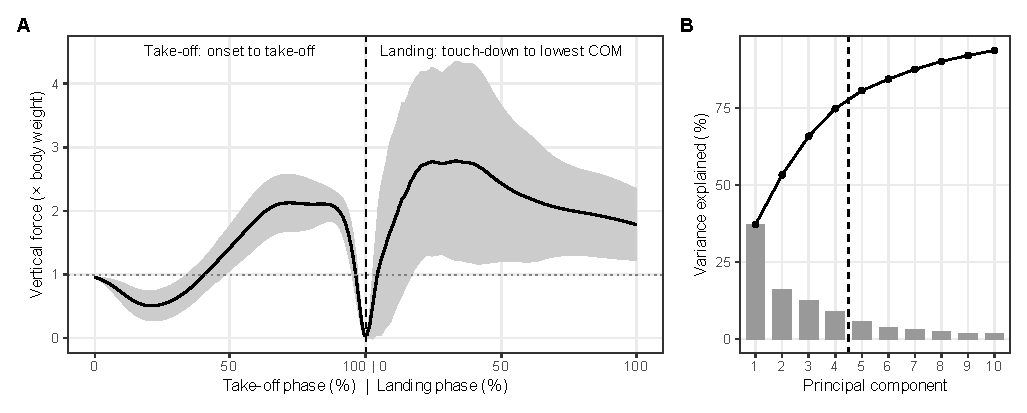
\includegraphics[width=\linewidth]{Fig1_mean_curve_scree}
\caption{\capMean}
\label{fig:mean}
\end{figure}

All four retained components were located almost entirely in the landing phase, which held \ldsPCD--\ldsPCB\% of their squared loadings (Table~\ref{tab:pcs}). PC1 (\varPCA\%) contrasted landings in which force rose to a large peak at about \peakPCA\% of the landing phase and remained well above body weight until the lowest point of the COM with landings in which force peaked early and then declined (Fig.~\ref{fig:pcs}). Its strongest correlate was landing duration ($r$~=~\rLdPCA): high scores denote short, stiff landings in which downward momentum is arrested quickly. PC1 was moderately related to peak landing force ($r$~=~\rLpfPCA) and essentially unrelated to contraction time ($r$~=~\rCtPCA) and countermovement depth ($r$~=~\rCmdPCA). PC2 to PC4 (\varPCB\%, \varPCC\% and \varPCD\%) described the timing and number of landing force peaks, contrasting single early peaks, single later peaks and double-peaked landings, with their largest loadings at \peakPCB\%, \peakPCC\% and \peakPCD\% of the landing phase. Peak landing force correlated with every component ($r$ = \lpfCorRange), whereas the correlations with contraction time and countermovement depth did not exceed \ctAbsMax{} and \cmdAbsMax{} in absolute value, and those with the vendor metrics did not exceed \vendorAbsMax.

% Generated by build2/mktab.py from the R pipeline output (tab3_components.tex); layout only.
\begin{table}[!htbp]
\centering
\begin{threeparttable}
\caption{Retained principal components (main analysis)}
\label{tab:pcs}
\footnotesize\setlength{\tabcolsep}{4pt}
\begin{tabular}{@{}l S[table-format=2.1] S[table-format=2.1] S[table-format=2.1] S[table-format=2.0] *{5}{S[table-format=-1.2]}@{}}
\toprule
 & {Variance} & {Cumulative} & {Landing} & {Peak} & \multicolumn{5}{c}{Pearson $r$ with} \\
\cmidrule(l){6-10}
Component & {(\%)} & {(\%)} & {share (\%)} & {at (\%)} & {LPF} & {JH} & {CT} & {CMD} & {LD} \\
\midrule
PC1 & 37.3 & 37.3 & 99.7 & 40 & 0.39 & 0.13 & -0.04 & 0.01 & -0.75 \\
PC2 & 16.0 & 53.3 & 99.9 & 26 & 0.22 & 0.13 & 0.02 & 0.00 & -0.14 \\
PC3 & 12.6 & 65.9 & 99.5 & 16 & 0.39 & 0.34 & 0.00 & -0.14 & -0.32 \\
PC4 & 8.9 & 74.8 & 99.3 & 9 & 0.45 & 0.24 & 0.15 & -0.18 & -0.04 \\
\bottomrule
\end{tabular}
\begin{tablenotes}[flushleft]\footnotesize
\item \textit{Note.} Landing share = percentage of the squared loading vector that lies in the landing block (the rest is in take-off). Peak at = position of the largest absolute loading, in \% of the landing phase. Signs are set so that the largest absolute loading is positive. LPF = peak landing force relative to body weight; JH = jump height; CT = contraction time; CMD = countermovement depth; LD = landing duration (touch-down to lowest COM).
\end{tablenotes}
\end{threeparttable}
\end{table}


\begin{figure}[tbp]
\centering
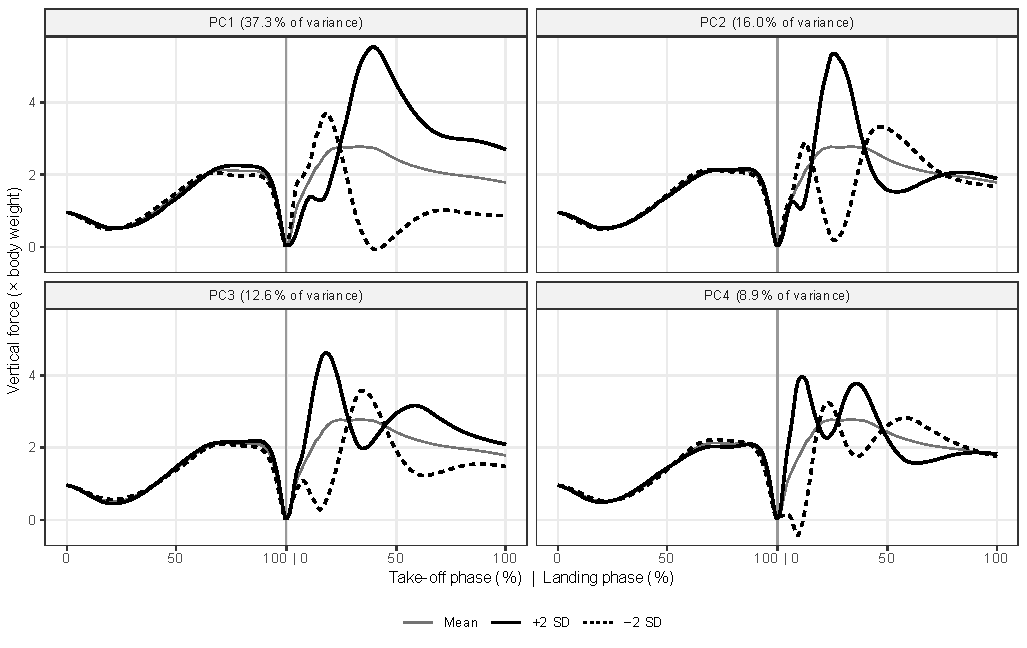
\includegraphics[width=\linewidth]{Fig2_pc_reconstructions_main}
\caption{\capPCs}
\label{fig:pcs}
\end{figure}

\subsection{Curve shape among trials matched on conventional metrics}

The jump-height band contained \jhBandN{} trials from \jhBandAth{} athletes with a jump height of \jhBandMean{} $\pm$ \jhBandSD{}\,cm, a standard deviation \jhBandSDfactor{} times smaller than that of the full sample. Within this band, take-off curves were similar, but landing curves differed widely (Fig.~\ref{fig:band}A). Matching on jump height reduced the dispersion of PC1 only modestly (ratio \jhRatioPCA, 95\% CI \jhLoPCA--\jhHiPCA), and the ratios for the other components ranged from \jhRatioOtherRange; every confidence interval included one (Table~\ref{tab:band}; Fig.~\ref{fig:band}B). The dispersion of the whole curve was unchanged (ratio \wholeJh). Matching on relative concentric peak force had no discernible effect (component ratios \rpfRatioRange; whole curve \wholeRpf). The result did not depend on the width of the band: across four band definitions, the PC1 ratio ranged from \bwPCARange, and all ratios from \bwAllRange.

% Generated by build2/mktab.py from the R pipeline output (tab4_bands.tex); layout only.
\begin{table}[!htbp]
\centering
\begin{threeparttable}
\caption{Score dispersion among trials matched on jump height or relative peak force}
\label{tab:band}
\footnotesize\setlength{\tabcolsep}{4pt}
\begin{tabular}{@{}l S[table-format=2.2] S[table-format=2.2] S[table-format=1.2] c S[table-format=2.2] S[table-format=1.2] c@{}}
\toprule
 & {Full sample} & \multicolumn{3}{c}{Jump-height band} & \multicolumn{3}{c}{Relative peak-force band} \\
\cmidrule(lr){3-5}\cmidrule(l){6-8}
Component & {SD} & {SD} & {Ratio} & 95\% CI & {SD} & {Ratio} & 95\% CI \\
\midrule
PC1 & 7.28 & 6.45 & 0.89 & {[0.70, 1.06]} & 7.33 & 1.01 & {[0.77, 1.16]} \\
PC2 & 4.77 & 4.62 & 0.97 & {[0.77, 1.16]} & 5.01 & 1.05 & {[0.82, 1.24]} \\
PC3 & 4.22 & 4.03 & 0.95 & {[0.74, 1.13]} & 4.25 & 1.00 & {[0.81, 1.17]} \\
PC4 & 3.56 & 4.16 & 1.17 & {[0.81, 1.44]} & 3.75 & 1.05 & {[0.87, 1.23]} \\
\addlinespace
Whole curve$^{a}$ & 11.92 & 11.99 & 1.01 & {} & 11.95 & 1.00 & {} \\
\bottomrule
\end{tabular}
\begin{tablenotes}[flushleft]\footnotesize
\item \textit{Note.} Bands contain the trials between the 45th and 55th percentiles of jump height (\jhBandLo--\jhBandHi\,cm; \jhBandN{} trials, \jhBandAth{} athletes) or of concentric peak force relative to body weight (\rpfBandLo--\rpfBandHi\,BW; \rpfBandN{} trials, \rpfBandAth{} athletes). Ratio = SD in the band divided by SD in the full sample; a ratio of 1 means that matching left the spread unchanged. CIs are percentile intervals from \nBoot{} athlete-level bootstrap resamples, conditional on the estimated components. Component SDs are in score units and are comparable only within this table. $^{a}$Square root of the summed point-wise variance of the 202-point curve.
\end{tablenotes}
\end{threeparttable}
\end{table}


\begin{figure}[tbp]
\centering
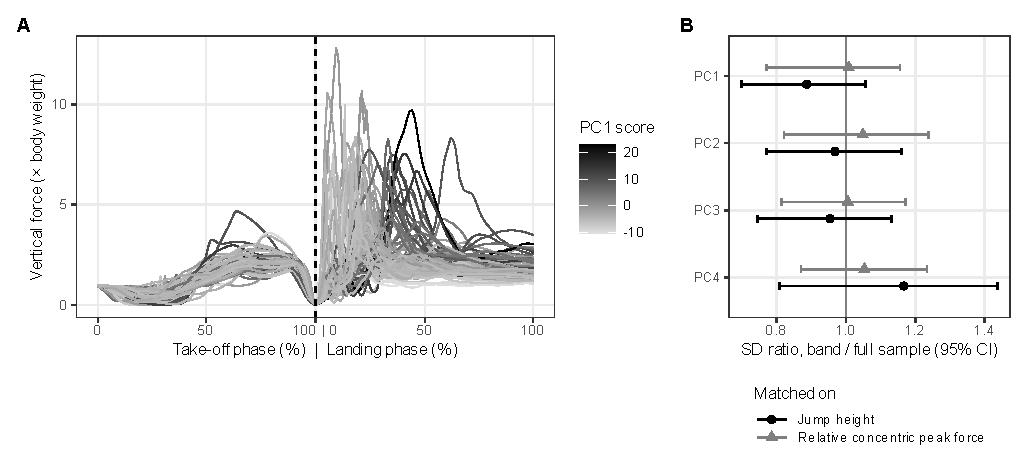
\includegraphics[width=\linewidth]{Fig3_matched_band}
\caption{\capBand}
\label{fig:band}
\end{figure}

\subsection{Variance explained by conventional metrics}

The four vendor metrics, age and body mass explained \rtwoRange\% of the variance of the retained components, leaving \unexplRange\% unexplained (Table~\ref{tab:r2}; Fig.~\ref{fig:r2}). Explained variance was lower under athlete-grouped cross-validation (\cvRange\%) and similar when one trial per athlete (\oneTrialRange\%) or athlete means (\athMeanRange\%) were analysed; the low values were therefore not a consequence of treating repeated trials as independent.

% Generated from package/output/paper_tables_latex/tab5_r2.tex (R pipeline); only layout changed.
\begin{table}[tbp]
\centering
\begin{threeparttable}
\caption{Variance of each component score explained by the four vendor metrics, age and body mass, and decomposition of component-score variance (main analysis).}
\label{tab:r2}
\footnotesize
\setlength{\tabcolsep}{2.5pt}
\begin{tabular*}{\linewidth}{@{\extracolsep{\fill}}lrrrrrrrr@{}}
\toprule
 & \multicolumn{5}{c}{$R^2$ on metrics, age and body mass (\%)} & \multicolumn{3}{c}{Variance of score (\%)} \\
\cmidrule(lr){2-6}\cmidrule(l){7-9}
Component & \makecell[r]{In-\\sample} & Adjusted & \makecell[r]{Athlete\\CV} & \makecell[r]{One trial\\per athlete} & \makecell[r]{Athlete\\means} & \makecell[r]{Between\\athletes} & \makecell[r]{Between\\sessions} & \makecell[r]{Within\\session} \\
\midrule
PC1 & 7.7 & 7.0 & 4.0 & 10.0 & 11.1 & 29.6 & 34.9 & 35.5 \\
PC2 & 2.7 & 2.0 & 0.3 & 4.3 & 5.4 & 21.4 & 17.0 & 61.6 \\
PC3 & 13.1 & 12.4 & 11.8 & 17.8 & 21.2 & 22.9 & 2.3 & 74.8 \\
PC4 & 9.1 & 8.4 & 6.3 & 11.1 & 13.8 & 10.0 & 20.3 & 69.6 \\
\bottomrule
\end{tabular*}
\begin{tablenotes}[flushleft]\footnotesize
\item \textit{Note.} Predictors: jump height, concentric peak force, eccentric braking impulse, concentric impulse over the first 100\,ms, age and body mass (ordinary least squares). In-sample and adjusted values use all \nTrials{} trials. Athlete CV = out-of-sample $R^2$ from five-fold cross-validation with athletes, not trials, allocated to folds. One trial per athlete = one randomly drawn trial per athlete (\nAth{} trials). Athlete means = scores and predictors averaged within athlete. Variance shares come from a three-level random-intercept model (athlete, session within athlete, trial within session) fitted by restricted maximum likelihood.
\end{tablenotes}
\end{threeparttable}
\end{table}


Between-athlete differences accounted for \betweenRange\% of the variance of the component scores, differences between sessions of the same athlete for \sessRange\%, and differences between trials within a session for \withinRange\% (Table~\ref{tab:r2}). PC1 was the most athlete-specific component (\betweenPCA\% between athletes, \sessPCA\% between sessions); for PC2 to PC4, \withinPCB\%, \withinPCC\% and \withinPCD\% of the variance arose between trials within the same session.

\begin{figure}[tbp]
\centering
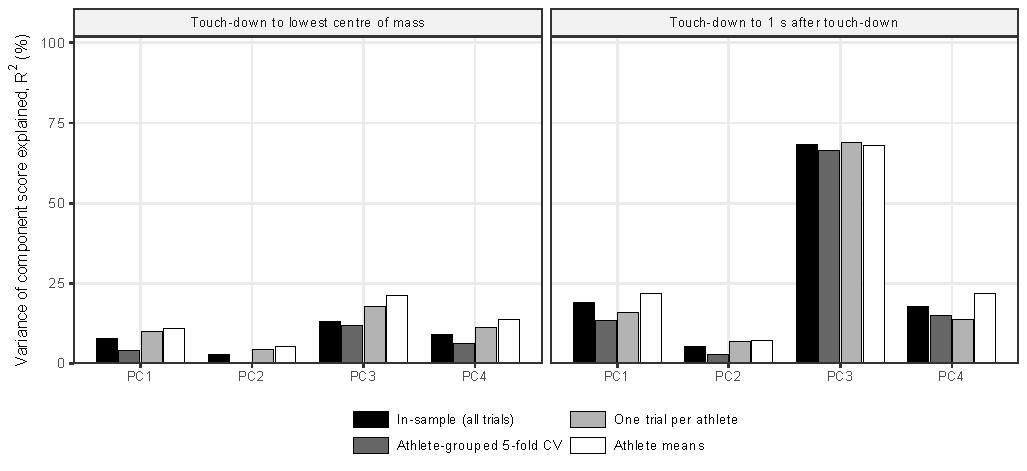
\includegraphics[width=\linewidth]{Fig4_variance_explained}
\caption{\capRtwo}
\label{fig:r2}
\end{figure}

\subsection{Sensitivity to the definition of the landing phase}

When the landing phase ended 1\,s after touch-down, the impact occupied only the first few per cent of the landing block and the remainder approximated quiet standing (Fig.~\ref{fig:window}). The four components then explained \cumFourS\% of the variance, and PC3 became a take-off component (\ldsSPCCtakeoff\% of its squared loading in the take-off phase) that was strongly related to contraction time ($r$~=~\rCtSPCC) and relative concentric peak force ($r$~=~\rRpfSPCC). This component was largely explained by the conventional metrics ($R^2$ = \rtwoSPCC\%; \cvSPCC\% under cross-validation), whereas the three landing components remained poorly explained ($R^2$ = \rtwoLandingSRange\%; Table~\ref{tab:window}; Fig.~\ref{fig:r2}). PC1 was again a landing component related to peak landing force ($r$~=~\rLpfSPCA) and landing duration ($r$~=~\rLdSPCA). Matching on jump height reduced PC1 dispersion somewhat more under this definition (ratio \jhRatioSPCA, 95\% CI \jhLoSPCA--\jhHiSPCA), but the dispersion of the whole curve was again unchanged (ratio \wholeJhS).

% Generated from package/output/paper_tables_latex/tab6_windows.tex (R pipeline); only layout changed.
\begin{table}[tbp]
\centering
\begin{threeparttable}
\caption{Main analysis compared with the sensitivity analysis in which the landing phase ended 1\,s after touch-down.}
\label{tab:window}
\footnotesize
\setlength{\tabcolsep}{3pt}
\begin{tabularx}{\linewidth}{@{}>{\raggedright\arraybackslash}Xll@{}}
\toprule
Quantity & \makecell[l]{Main: landing to\\lowest COM} & \makecell[l]{Sensitivity:\\1-s landing} \\
\midrule
Trials / athletes after QC & 805 / 212 & 811 / 212 \\
Variance explained, PC1--PC4 (\%) & 37.3, 16.0, 12.6, 8.9 & 20.2, 16.6, 15.1, 10.2 \\
Cumulative, PC1--PC4 (\%) & 74.8 & 62.2 \\
Landing share of loading, PC1--PC4 (\%) & 99.7, 99.9, 99.5, 99.3 & 96.4, 92.5, 3.7, 80.2 \\
PC1 SD ratio, jump-height band (95\% CI) & 0.89 (0.70--1.06) & 0.82 (0.69--0.96) \\
Whole-curve SD ratio, jump-height band & 1.01 & 1.01 \\
In-sample $R^2$, PC1--PC4 (\%) & 7.7, 2.7, 13.1, 9.1 & 19.1, 5.3, 68.3, 17.8 \\
Athlete-CV $R^2$, PC1--PC4 (\%) & 4.0, 0.3, 11.8, 6.3 & 13.4, 2.8, 66.4, 15.1 \\
Between-athlete variance, PC1--PC4 (\%) & 29.6, 21.4, 22.9, 10.0 & 45.3, 18.7, 26.5, 31.6 \\
$r$(PC1, landing peak force) & 0.39 & 0.71 \\
$r$(PC3, contraction time) & 0.00 & $-$0.79 \\
\bottomrule
\end{tabularx}
\begin{tablenotes}[flushleft]\footnotesize
\item \textit{Note.} COM = centre of mass; CI = confidence interval; CV = cross-validation. Between-athlete variance is taken from the three-level random-intercept model. In the 1-s window PC3 is a take-off component (Fig.~\ref{fig:window}), which explains its correlation with contraction time.
\end{tablenotes}
\end{threeparttable}
\end{table}


\begin{figure}[tbp]
\centering
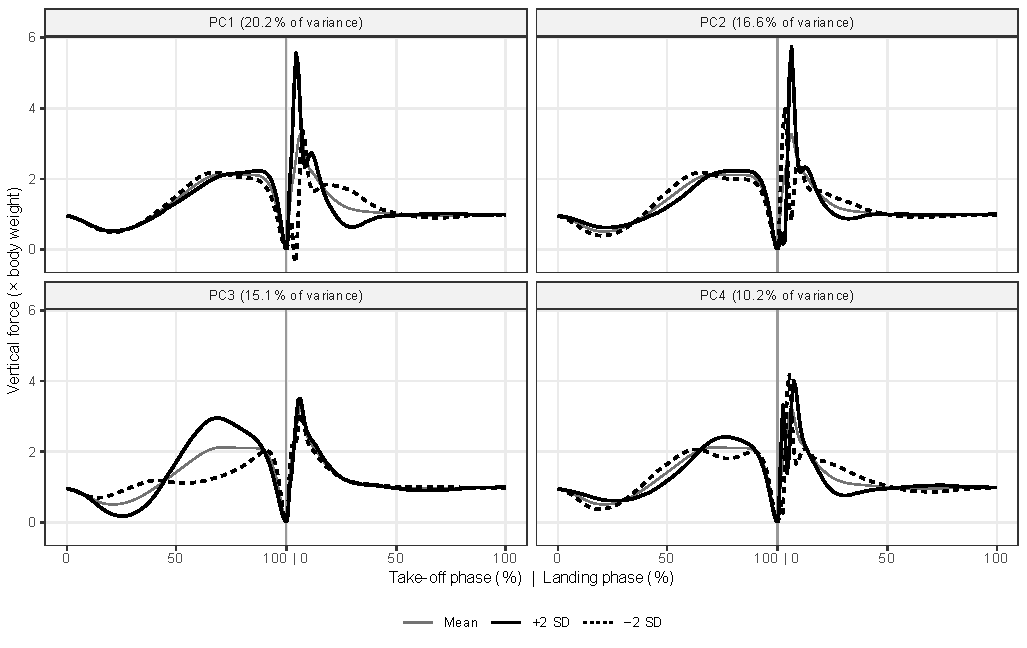
\includegraphics[width=\linewidth]{Fig5_pc_reconstructions_1s}
\caption{\capWindow}
\label{fig:window}
\end{figure}

\section{Discussion}
\label{sec:discussion}

\subsection{Principal findings}

This study examined whether countermovement jumps that score alike on conventional force-plate metrics also resemble one another in the shape of the force--time curve, and how much of that shape the metrics capture. Three findings emerge. First, when take-off and landing are analysed together, the dominant modes of variation lie in the landing, and the first describes how quickly the athlete arrests the fall. Second, jumps matched closely on jump height, or on relative peak force, were scarcely more alike in curve shape than jumps in general. Third, jump height, concentric peak force, eccentric braking impulse, early concentric impulse, age and body mass together explained no more than \rtwoPCC\% of the variance of any landing component, and less under cross-validation. Equal scores on these metrics therefore do not imply an equivalent jump. A further finding qualifies the interpretation of the components as strategies: most of their variance arose within athletes, between sessions and between trials of the same session.

\subsection{Relation to previous research}

The results are consistent with earlier evidence that discrete force-plate variables summarise the jump incompletely. \textcite{dowling1993} found that no single kinetic or temporal variable explained vertical jump performance well, \textcite{richter2014b} showed that dimensionality-reduction techniques captured performance-related features of the jump better than discrete points, and principal component waveform analysis has been used to identify features of the curve associated with improvements in performance \parencite{floria2019}. These studies, like most CMJ waveform analyses \parencite{cormie2009,sole2018,harry2018}, examined the propulsive part of the jump and asked how curve features relate to performance. The present study reverses the question and asks how much of the curve the performance metrics account for. The matched-band analysis offers a direct answer to this question because it holds jump height almost constant and observes the variation that remains.

The sensitivity analysis clarifies where the unexplained variation lies. With the 1-s landing window, a take-off component emerged that described the duration and amplitude of the propulsive force and of which approximately two-thirds was explained by the conventional metrics. This is consistent with the close relationships between contraction time, relative peak force, impulse and jump height that follow from impulse--momentum mechanics \parencite{linthorne2001,mcmahon2018}, and with the distinction drawn between performance metrics and strategy variables \parencite{harry2024}. The metrics that practitioners usually report thus appear to be reasonable summaries of the take-off but convey little about the landing. Because the four vendor metrics were designed to describe propulsion, this result should not be interpreted as a deficiency of those metrics; rather, it indicates that the landing recorded in every trial contains substantial information that routine reports omit.

The prominence of the landing is consistent with the wider literature. Landings that arrest the body quickly with high forces have been linked to injury risk in young female athletes \parencite{leppanen2017}, and landing kinetics have some utility as predictors of injury \parencite{pedley2020}. PC1, which separated short, stiff landings from longer and more compliant ones, corresponds closely to this construct. Its relation to landing duration follows from impulse--momentum principles: because the landing phase in the main analysis ends when the downward velocity reaches zero, the mean force over the phase is determined by the touch-down velocity and the duration of the landing, so that a shorter landing must be accompanied by higher forces. The weaker correlation with peak landing force indicates that the component describes the time course of force rather than its maximum alone.

\subsection{Trial-to-trial variability and the interpretation of strategies}

Between-athlete differences accounted for at most \betweenPCA\% of the variance of any component, which corresponds to poor single-trial reliability by conventional benchmarks \parencite{koo2016}, and for PC2 to PC4 most of the variance arose between trials of the same session. The landing differences among jumps matched on jump height therefore appear to reflect, to a large extent, how a given athlete landed on a given trial rather than a fixed characteristic of that athlete. This interpretation accords with the view that movement variability is an intrinsic and often functional feature of skilled performance \parencite{davids2003,bartlett2007,preatoni2013}, and with the known sensitivity of CMJ variables to the number of trials and to protocol details \parencite{cormack2008,heishman2020}. Landing behaviour is also likely to depend on instructions and perceived effort \parencite{hite2025}, which were not standardised for landing in routine testing. The term \emph{strategy} should therefore be understood here as the manner in which a trial was executed; whether athletes possess stable landing strategies can be established only from repeated, standardised landings.

\subsection{Methodological considerations}

Two analytical choices had a considerable influence on the results and merit reporting in any similar study. The first is the definition of the end of the landing. Ending the landing at the lowest point of the COM confines the landing block to impact absorption and makes landing timing comparable across trials, whereas a fixed window devotes most of the block to quiet standing and compresses the impact into a few points; this lowered the variance captured by four components from \cumFour\% to \cumFourS\% and altered the composition of the components. The second is the scaling of the curve. Covariance PCA of body-weight-normalised force weights each part of the curve in proportion to its variance; because landing forces are larger and more variable than take-off forces, the take-off contributes little to the leading components unless the landing is short or analysed separately. Neither choice is inherently preferable, but the two address different questions, and the matched-band and regression results should be interpreted accordingly. Alignment on further events, such as the landing force peak \parencite{moudy2018}, functional PCA \parencite{ramsay2005,warmenhoven2019} and statistical parametric mapping \parencite{pataky2013} are natural extensions.

\section{Managerial and practical implications}
\label{sec:implications}

The findings have four implications for practitioners and for those who manage athlete-monitoring programmes. First, two athletes with the same jump height may land very differently; ranking or grouping athletes on jump height alone therefore conceals differences in landing mechanics. Second, the landing is recorded in every CMJ at no additional cost, and simple landing descriptors, in particular landing duration to the lowest point of the COM and peak landing force relative to body weight, capture much of the dominant landing component and could be added to routine reports. Third, because landing shape varied considerably between trials, decisions should be based on the mean of several trials, or on repeated sessions, rather than on a single landing. Fourth, unusual landing curves should prompt closer observation of how an athlete lands, under standardised instructions, rather than a diagnosis, since their relationship with injury in footballers has not been established.

More generally, the study illustrates a point relevant to organisations that rely on instrumented measurement. The summary indicators produced by commercial software are a design choice, and in these data they retained most of the information about the take-off but little about the landing. Applying a standard dimensionality-reduction technique to data that were already collected revealed variation that the routine indicators did not capture. Programme managers who invest in measurement systems may therefore benefit from periodically examining the full recorded signal before settling on a fixed set of reported indicators, while recognising, as these results show, that additional variation is useful for decisions only if it is reproducible across trials.

\section{Limitations and directions for future research}
\label{sec:limitations}

Several limitations should be noted. Landing was not standardised in routine testing, so part of its variation may reflect instructions, habits or effort rather than neuromuscular capacity. The end of the landing depends on body mass and on a velocity estimated from flight time, both of which carry error \parencite{street2001}, and it could not be identified in \nLowcomMissing{} trials. The sample comprised male footballers from a single centre over a wide age range (\ageMin--\ageMax{} years), most of them adolescents. Maturity status was not recorded, although growth and maturation affect jump performance in youth athletes \parencite{malina2015,lloyd2012}, and the results may not generalise to female athletes, to other sports or to other age groups. The regressions were linear and used four metrics; other vendor variables, including landing variables, would explain more of the landing components, and non-linear models might explain somewhat more, although the weak correlations suggest that the gain would be limited. PCA on linearly time-normalised curves combines differences in timing and in amplitude. Finally, the number of components was fixed in advance rather than selected from the data; this avoids tuning but means that the remaining components, which together explained about a quarter of the variance, were not interpreted.

Future studies could examine whether landing components are stable when landings are standardised and repeated, relate them to injury, fatigue and return-to-play outcomes in prospective designs, and extend the analysis to female athletes and other sports. Separate analysis of take-off and landing, registration on additional events, and functional or multivariate methods that combine curve shape with timing would help to distinguish strategy from execution variability. Establishing reference values for landing components across age and maturity would make this information usable in routine monitoring.

\section{Conclusion}
\label{sec:conclusion}

In male footballers, countermovement jumps matched closely on jump height, or on relative peak force, differed almost as much in the shape of their force--time curves as jumps in general. The dominant differences lay in how athletes absorbed the landing, above all in how quickly the fall was arrested, and the four conventional vendor metrics, together with age and body mass, explained little of them. These differences were, however, largely trial-specific. The landing phase of the CMJ, which is recorded in every trial but rarely reported, provides information that conventional take-off metrics do not, and it merits inclusion in routine force-plate reports, provided that it is interpreted over repeated trials.

\nolinenumbers

\section*{Declarations}
\subsection*{Declaration of competing interest}
The authors declare that they have no known competing financial interests or personal relationships that could have appeared to influence the work reported in this paper.
\subsection*{Funding}
This research did not receive any specific grant from funding agencies in the public, commercial or not-for-profit sectors.
\subsection*{Data availability}
The raw force-plate exports are owned by the testing centre and were provided under a non-disclosure and data-sharing agreement; they cannot be shared publicly. The analysis code is available from the corresponding author on request, and de-identified trial-level data may be made available on reasonable request, subject to the permission of the data owner. (Repository details are withheld for anonymous review and are given on the title page.)
\subsection*{Declaration of generative AI and AI-assisted technologies in the writing process}
During the preparation of this work, the authors used AI tools to assist with language editing and code review. After using these tools, the authors reviewed and edited the content as needed and take full responsibility for the content of the publication.

\singlespacing
\printbibliography
\end{document}
